% Metódy inžinierskej práce

\documentclass{article}

%\usepackage[T1]{fontenc}
\usepackage[IL2]{fontenc} % lepšia sadzba písmena Ľ než v T1
\usepackage[utf8]{inputenc}
\usepackage{graphicx}
\usepackage{url} % príkaz \url na formátovanie URL
\usepackage{hyperref} % odkazy v texte budú aktívne (pri niektorých triedach dokumentov spôsobuje posun textu)
\usepackage{enumitem}  % For adjusting list spacing
\usepackage{indentfirst}
\usepackage{amsmath}
\usepackage{float}
\usepackage{tabularx}
\usepackage{array}
\usepackage{booktabs}
\usepackage{multirow}
\usepackage{multicol}
\usepackage{xcolor}

\usepackage{cite}
%\usepackage{times}
\usepackage{caption}
\captionsetup{labelsep=period}

\pagestyle{headings}

\title{Content-based filtering\thanks{Semester project in the subject Methods of engineering work. Year 2024/25, supervision: Pavol Baťalík}}

\author{Sladkovskyi Heorhii\\[2pt]
	{\small Slovak University of Technology in Bratislava}\\
	{\small Faculty of Informatics and Information Technologies STU in Bratislava}\\
	{\small \texttt{xsladkovskyi@stuba.sk}}
	}

\date{\small 3. october 2024}



\begin{document}

\maketitle
\tableofcontents

%\section*{Reference Papers}\label{sec:reference_papers}


\begin{enumerate}[noitemsep, topsep=1px]
    \item \href{https://dl.acm.org/doi/10.1145/3610548.3618189}{Content-based Search for Deep Generative Models} 
    \item \href{https://dl.acm.org/doi/10.1145/2611286.2611300}{Content-based filtering discovery protocol (CFDP): scalable and efficient OMG DDS discovery protocol}
    \item \href{https://dl.acm.org/doi/10.1145/2661829.2661940}{Social Book Search Reranking with Generalized Content-Based Filtering}
    \item \href{https://dl.acm.org/doi/10.1145/2501025.2501036}{Customized reviews for small user-databases using iterative SVD and content based filtering}
    \item \href{https://dl.acm.org/doi/10.1145/1277741.1277903}{A multi-criteria content-based filtering system}
    \item \href{https://dl.acm.org/doi/10.1145/1015330.1015394}{Unifying collaborative and content-based filtering}
    \item \href{https://dl.acm.org/doi/10.1145/544220.544341}{Content-based filtering and personalization using structured metadata}
    \item \href{https://dl.acm.org/doi/10.1145/2492517.2500283}{Recommender system by grasping individual preference and influence from other users}
\end{enumerate}

Springer link
\begin{enumerate}[noitemsep, topsep=1px]
    \item \href{https://link.springer.com/chapter/10.1007/978-981-97-0538-2_3}{Collaborative Filtering and Content-Based Systems}
    \item \href{https://link.springer.com/chapter/10.1007/978-3-031-35078-8_37}{Movie Recommendation Using Content-Based and Collaborative Filtering Approach}
    \item \href{https://link.springer.com/chapter/10.1007/978-3-031-59707-7_9}{Sentiment Analysis and Innovative Recommender System: Enhancing Goodreads Book Discovery Using Hybrid Collaborative and Content Based Filtering}
    \item \href{https://link.springer.com/chapter/10.1007/978-3-031-34622-4_13}{Integrated Music Recommendation System Using Collaborative and Content Based Filtering, and Sentiment Analysis}
    \item \href{https://link.springer.com/chapter/10.1007/978-981-99-2287-1_50}{Personalized Recommendation of Literature Resources in University Library Based on Abstract Content Filtering Algorithm}
    \item \href{https://link.springer.com/chapter/10.1007/978-981-16-2594-7_47}{Job Recommendation System Using Content and Collaborative-Based Filtering} 
    \item \href{https://link.springer.com/chapter/10.1007/978-981-19-7660-5_8}{Development of Hybrid Personalized E-commerce Using Collaborative Filtering and Content-Based Filtering for South Cartel Clothing Company}
    \item \href{https://link.springer.com/chapter/10.1007/978-3-031-19958-5_98}{A Hybrid Hotel Recommendation Using Collaborative, Content Based and Knowledge Based Approach}
\end{enumerate} %TODO : temp, only for development
\begin{abstract}
    \ldots
\end{abstract}
\newpage %TODO : temp, only for development
\section{Introduction}\label{sec:introduction}

\subsection{Definition}% Definition of Content-Based Filtering | DRAFT, TODO : change the name

\subsection{Importance in recommendation systems} %TODO

\subsection{Overview} %TODO
\section{Algorithms for content-based filtering}\label{sec:cbf_algorithms}
Content-based filtering could be used in a variety of contexts. Depending on the needs of a recommendation system we could have different implementations of CBF. Depending on data type, it comonly used models include Term frequency–inverse document frequency (TF-IDF)\cite{TF_IDF}, Naive Bayes classifier \cite{Naive_classifier}, k-Nearest Neighbors or neural networks. The most popular and widely methods are based on vector 

\subsection{Decision-tree method}
Decision-tree could be used not only with content-based filtering, but also with other recommendation methods. It is not really popular due to several reasons, but could have advantages in specific situations. Decision-tree method relies on inductive learning, therefore we firstly should have some data from the user (his preferences or previous actions). After that, we could use algorithms like C4.5\cite{C4_5} or newer version C5.0. Given algorithm will produce a decision tree based on user preferences and it will be used as a user profile. The example of a decision tree is shown in Figure~\ref{fig:decision_tree}\cite{Decision_Tree}.

After construction of the decision tree, we can classify new items, with which the user has not yet interacted. If the item has similar categories (this approach could be used only if items have some sort of categorization) to those which are preferable to user profile, the output of the decision tree for these items would be abstract “Like”. This will mean that we could recommend a new item to a user with a high probability that this item will interest the user. The decision tree can be reconstructed during the process of interacting with new content which will improve the recommendation results.

However, this algorithm has some disadvantages. Firstly, the computational complexity of C4.5 during the training data is $\mathbf{O(m^2)}$. For a small amount of data it wouldn't be a problem, but if the user is interacting with thousands of items, rebuilding the decision tree won't be a trivial task. Computational cost during the recommendation process is $\mathbf{O(n)}$, which also could be a problem with high amounts of presented items\cite{Decision_Tree}.
\begin{center}
    \begin{figure}[H]
    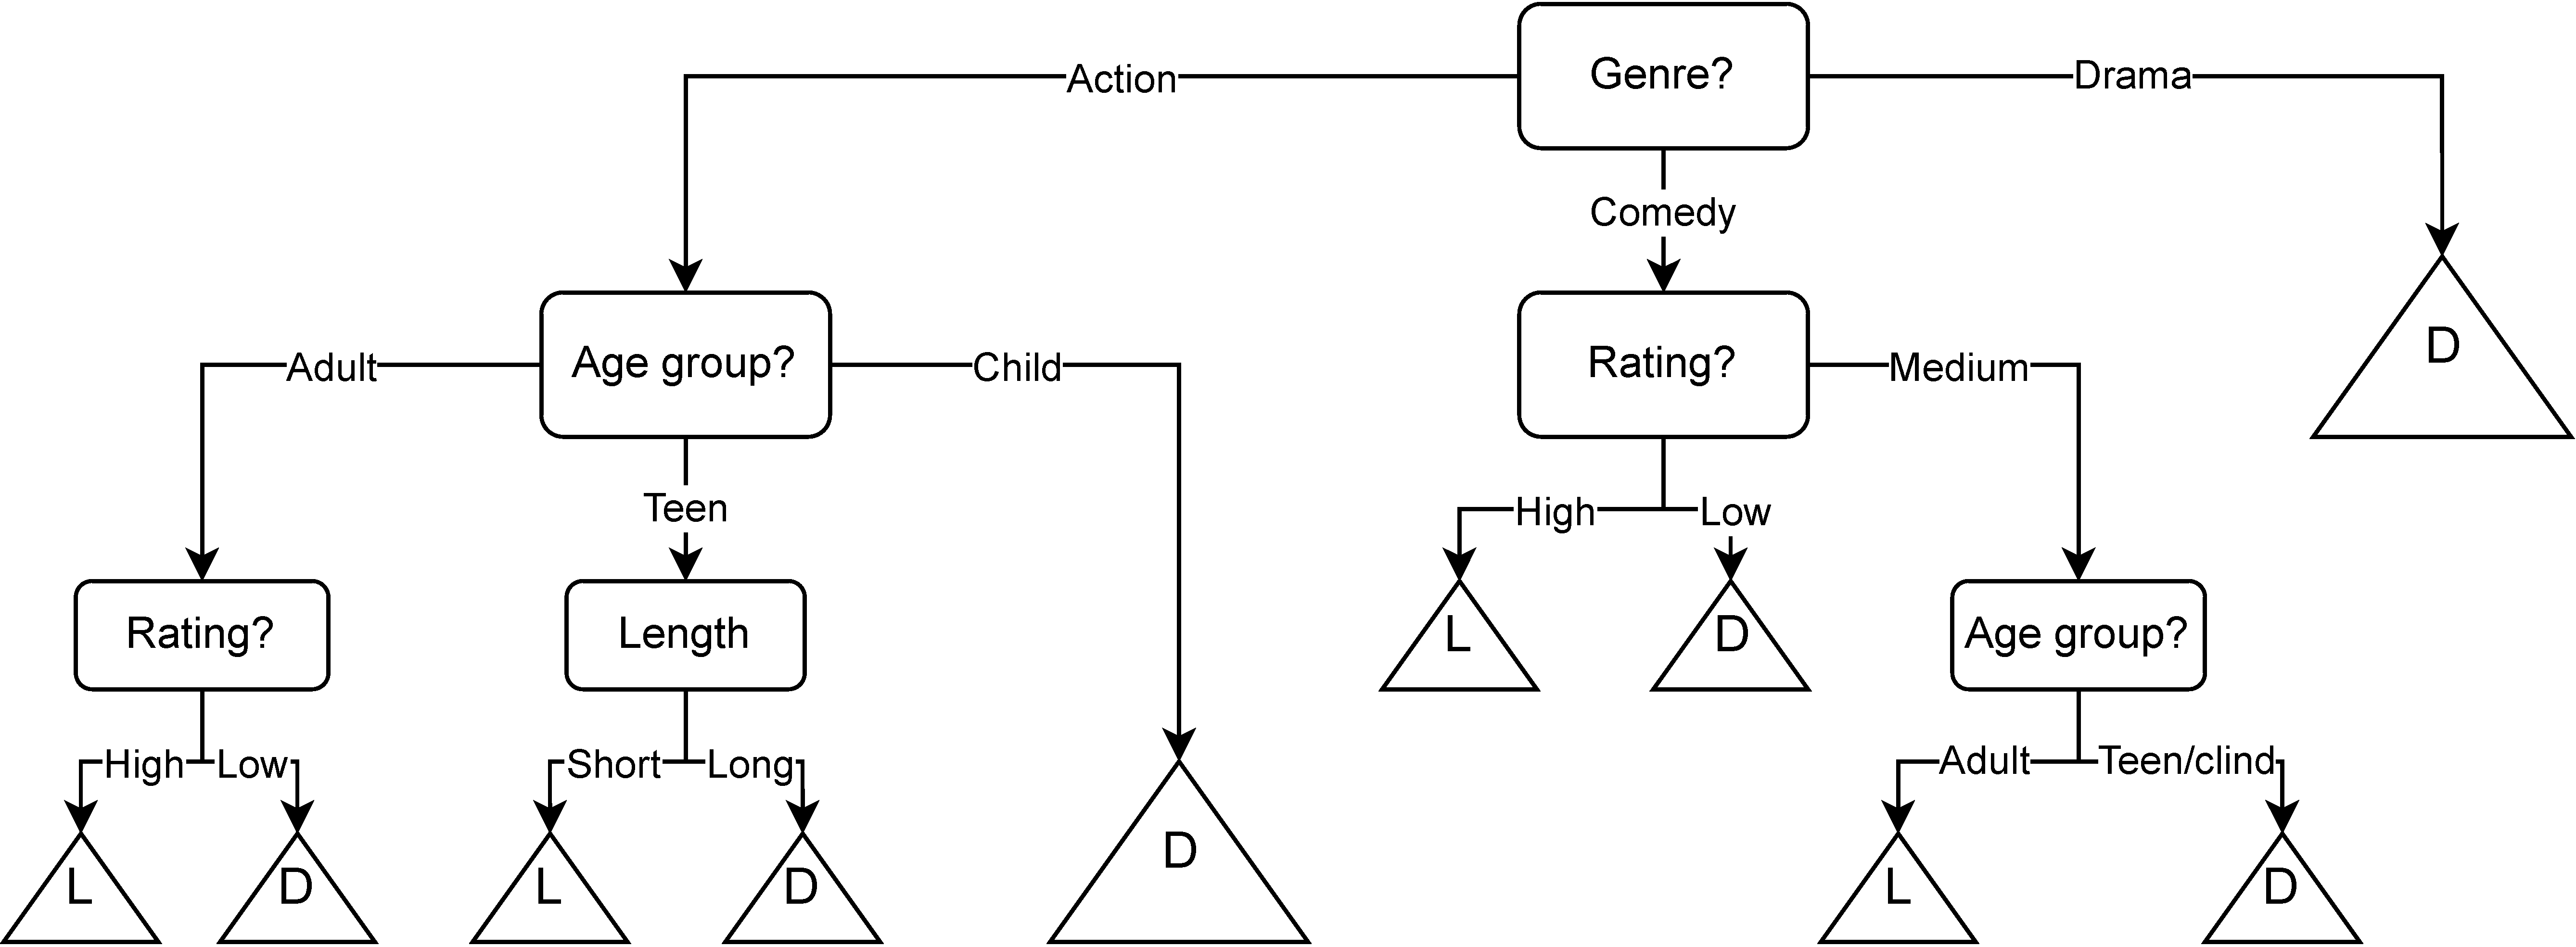
\includegraphics[width=\textwidth]{figures/diagrams/article_decision_tree.pdf}
    \caption{Example of decision-tree}
    \label{fig:decision_tree}
    \end{figure}
\end{center}

\subsection{K-Nearest Neighbor method}
K-Nearest Neighbor (KNN) belongs to vector space methods that are used in N dimensional environments (see section 3 for more details). It is highly used and has better results than decision-tree in the majority of data sets\cite{KNN}.

But before using KNN, we should collect data from user interactions (e.g. user likes) into a user-item matrix. The example of the user-item matrix is shown in Figure 2. In example, user has different amount of 

\begin{table}[h]
    \centering
    \begin{tabular}{|c|c|c|c|c|}
        \hline
        \textbf{Users} & \textbf{Movie 1} & \textbf{Movie 2} & \textbf{Movie 3} & \textbf{Movie 4} \\        
        \hline
        User 1 & 3 & 0 & 1 & 2\\
        \hline
        User 2 & 0 & 5 & 5 & 3\\
        \hline
        User 3 & 5 & 1 & 1 & 2\\
        \hline
        User 4 & 0 & 0 & 5 & 0\\
        \hline
    \end{tabular}
    \caption{User-item matrix}\label{tab:user_item_matrix}
\end{table}

\begin{table}[h]
    \centering
    \begin{tabular}{|c|c|c|c|c|}
        \hline
        \textbf{Genres} & \textbf{Movie 1} & \textbf{Movie 2} & \textbf{Movie 3} & \textbf{Movie 4} \\        
        \hline
        Action  & 1 & 0 & 0 & 1\\
        \hline
        Romance & 0 & 1 & 1 & 0\\
        \hline
        Comedy  & 1 & 1 & 1 & 0\\
        \hline
        Horror  & 0 & 0 & 0 & 1\\
        \hline
    \end{tabular}
    \caption{Genre-movie matrix}\label{tab:genre_movie_matrix}
\end{table}

\newcommand{\cosinesimilarity}{%
    \begin{equation}
    \text{similarity} = \cos(\theta) = \frac{\vec{A} \cdot \vec{B}}{||\vec{A}|| \times ||\vec{B}||} = \frac{\sum_{i=1}^{n} A_i B_i}{\sqrt{\sum_{i=1}^{n} A_i^2} \times \sqrt{\sum_{i=1}^{n} B_i^2}}
    \end{equation}
}
\begin{table}[h]
    \centering
    \begin{tabular}{|c|c|c|c|c|}
        \hline
         & Movie 1 & Movie 2 & Movie 3 & Movie 4 \\        
        \hline
        Movie 1 &1		&0.5	&0.5	&0.5\\
        \hline	
        Movie 2 &0.5	&1      &1		&0	\\
        \hline
        Movie 3 &0.5	&1		&1		&0	\\
        \hline
        Movie 4 &0.5	&0		&0		&1	\\
        \hline
    \end{tabular}
    \caption{Cosine similarity matrix}\label{tab:cosine_similarity_matrix}
\end{table}
\section{Data representation in content-based filtering}\label{sec:cbf_data_rep}

\subsection{Data extraction} %TODO

\subsection{Data unification using embeddings} %TODO

\subsection{Advantages of embeddings in CBF} %TODO
\section{Advantages and disadvantages of content-based filtering}\label{sec:cbf_advantages_disadvantages} %TODO : could be rewrited to usecases of CBF

\subsection{Advantages} %TODO

\subsection{Limitations} %TODO

 %TODO : temp, could be removed
\section{Comparison of CBF with other recommendation methods}\label{sec:cbf_comparison}

\section{Advantages and disadvantages} %TODO : temp, could be removed

\subsection{Collaborative filtering vs. content-based filtering} %TODO : rewrite name

\subsection{Hybrid Models} %TODO
\section{Use cases}\label{sec:usecases} % TODO : change the name

\subsection{Media streaming platforms} %TODO

\subsection{News} %TODO

\subsection{E-commerce} %TODO
\section{Conclusion}\label{sec:conclusion}

\nocite{*} %TODO : temp

\bibliography{bibliography/references}
\bibliographystyle{unsrt}
\end{document}
